\chapter{Plugin functioning}
\label{app:B}
In this Appendix we outline how the plugin works to highlight how \textit{sign-to-contract} was integrated.
We aim to give an overview on which are the difficulties that arise when integrating this scheme in a signing software, while avoiding to focus on the complications related to where we decided to set our implementation.
Note that although \textit{sign-to-contract} per se is not extremely complicated, the workaround to use it to timestamp involves actions related to very disparate contexts: hashing the file, communicate with network, create a bitcoin transaction, extract the key from the wallet, perform elliptic curve math, properly encode the signature and then the transaction, broadcast the transaction, retrieve the information to complete the proof and finally correctly serialize the timestamp.
Explaining in details how all those actions are performed goes beyond the purpose of this work, for a deeper analysis, examine the code. We proceed by illustrating the plugin functioning, use Figure \ref{fig:plugin-scheme} to follow the description. 

The procedure is divided in 5 steps, \verb|Add New File|, \verb|Create New TX|, \verb|S2C|, \verb|Send TX| and \verb|Upgrade|. 
When running the application, each of these steps needs some action to be performed and a button to be pressed, in this sense they pause the flow of the procedure.

At first stage, it is possible to add new files to timestamp. 
They are included in a support database: it is stored their path and the corresponding incomplete proof, which, at this phase, is the file hash. 
In the following steps, the proof is extended with the new operations that are applied to the hash value.

The second phase consists in creating a new transaction. 
Once chosen the destination for the coins, it is performed a coin selection among the UTXOs in the wallet, the result is an unsigned transaction $uTX$. 

Then one may sign $uTX$ in the standard way, by pressing \verb|sign|, or with \textit{sign-to-contract}, pressing \verb|S2C|. 
If the latter is chosen, all the files to timestamp in the database are salted and then committed in a Merkle tree, with tip $MT$.
The operations of each branch are appended to the corresponding proof, as a result all the proofs lead to $MT$.
Then the actual \textit{sign-to-contract} procedure is implemented, the private key is retrieved from the wallet, $uTX$ is signed with contract $MT$, generating the singed transaction $TX$.

When $TX$ is broadcast to the network, the proofs are extended until its TXID.
Then, it is necessary to wait until $TX$ is confirmed, that is when it is at least 6 blocks deep. 

Finally the upgrade phase can be performed: the Merkle path, from the TXID to the block header Merkle root, is retrieved from the network and appended to the incomplete proofs, turning them into legit timestamps.
Next to each file to timestamp is placed a \verb|.ots| file which is the serialized timestamp.

\begin{figure}
	\begin{center}
		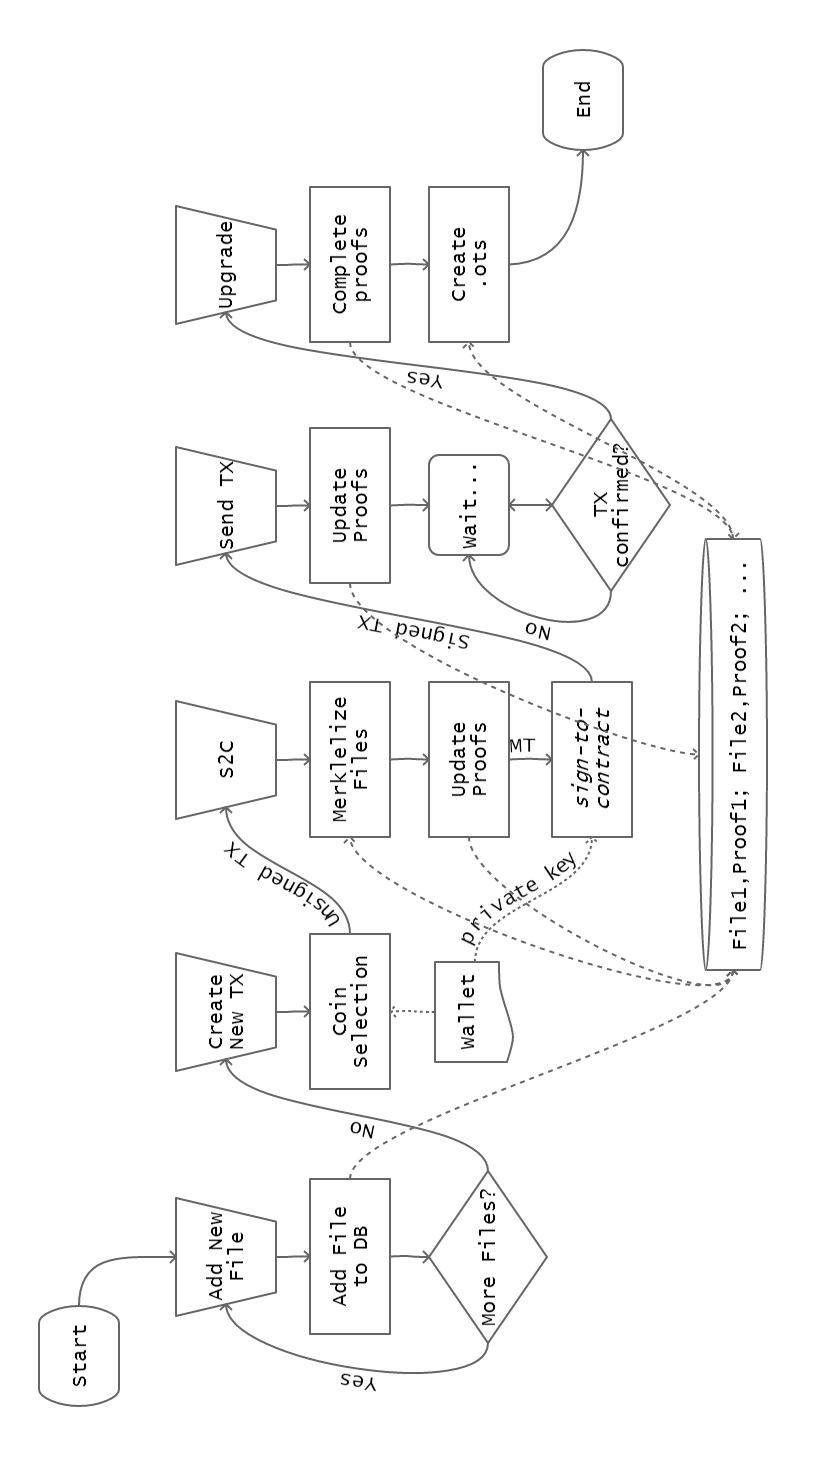
\includegraphics[width=0.75\linewidth]{Images/plugin-working.png}
		\caption[Simplified scheme of the Electrum plugin]{Simplified scheme of the Electrum plugin for \textit{sign-to-contract}.}
		\label{fig:plugin-scheme}
	\end{center}
\end{figure}